% ==============================================================================
% 第 6 章：分类与结构体 (Chapter 6: Itemizations and Structures)
% ==============================================================================

\chapter{分类与结构体}
\label{sec:ch06_itemizations}

在第 4 章中，我们学习了\term{分类数据}（Itemizations），它通过将离散的原子值（如字符串标签）和连续的范围（如数值区间）组合在一起来描述复杂情况。在第 5 章中，我们学习了\term{结构体}（Structures），它允许我们将多项相互关联的数据打包为一个单一的复合实体。

本章将这两大核心概念融合在一起：\textbf{带有结构体的分类数据}。在实际软件工程中，这种组合模式无处不在。一个系统在不同阶段可能处于截然不同的状态模式，而每种状态模式所需追踪的复合属性也大相径庭。例如在视频游戏中，玩家在未发射子弹前只需记录飞船位置，发射子弹后则必须同时追踪飞船与子弹的位置。

此外，本章还将系统性地探讨\term{输入验证}（防御性设计）、\term{世界状态谓词}以及\term{相等性比较谓词}，使我们的程序不仅结构严谨，更具备工业级的鲁棒性。

% ==============================================================================
\section{再论分类数据的设计}
\label{sec:6.1_designing_with_itemizations_again}
% ==============================================================================

为了掌握带有结构体的分类数据设计，我们将深入开发一个经典的街机游戏——\term{太空侵略者}（Space Invaders）。

在游戏中，一架不明飞行物（UFO）自天顶向地面降落，地面上一辆坦克（Tank）左右移动并伺机发射一枚反击导弹（Missile）。游戏存在两个截然不同的状态阶段：
\begin{enumerate}
  \item \textbf{瞄准阶段（Aiming）}：导弹尚未发射，装载在坦克上；
  \item \textbf{发射阶段（Fired）}：导弹已点火发射，正垂直向天空疾驰。
\end{enumerate}

\begin{figure}[htbp]
  \centering
  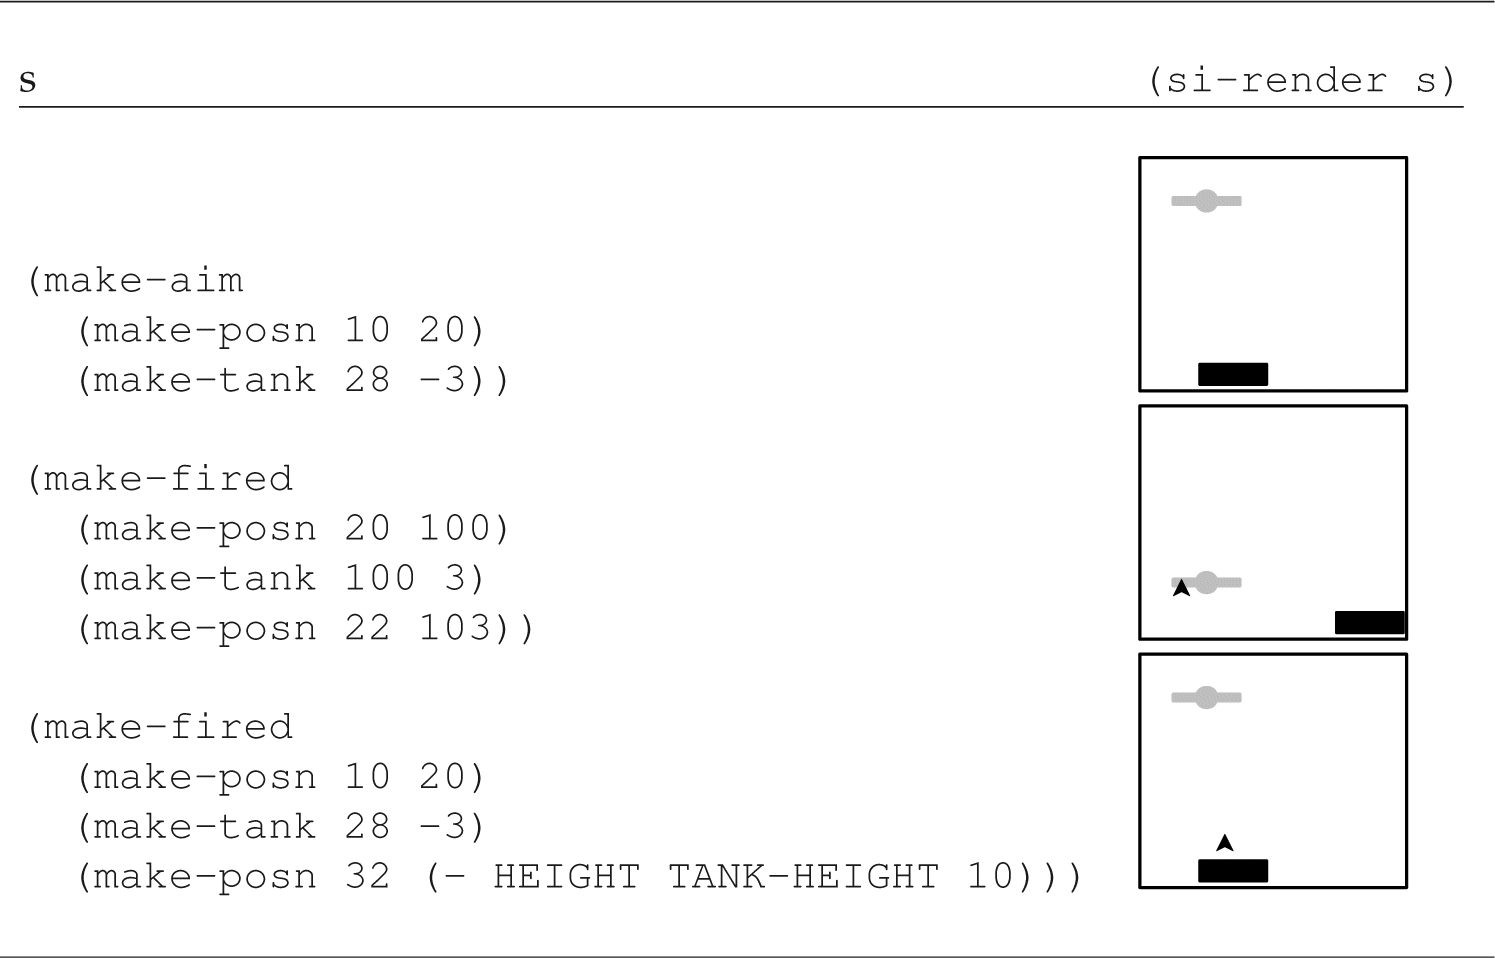
\includegraphics[width=0.75\textwidth]{images/00118.png}
  \caption{太空侵略者游戏状态渲染示例}
  \label{fig:space_invader_render_examples}
\end{figure}

针对这两个状态分支，我们定义两个专属的结构体：

\begin{lstlisting}[language=BSL]
(define-struct aim [ufo tank])
(define-struct fired [ufo tank missile])
\end{lstlisting}

进而定义游戏状态分类数据 \code{SIGS}（Space Invader Game State）：

\begin{lstlisting}[language=BSL]
; 一个 SIGS (太空侵略者游戏状态) 是以下两者之一：
; -- (make-aim Posn Tank)
; -- (make-fired Posn Tank Posn)
; 解释：表示游戏处于“未发射导弹”或“导弹已发射”状态。
; 其中 Posn 表示 UFO 或导弹在画布上的坐标；
; Tank 记录坦克的水平位置与移动速度。
\end{lstlisting}

\begin{figure}[htbp]
  \centering
  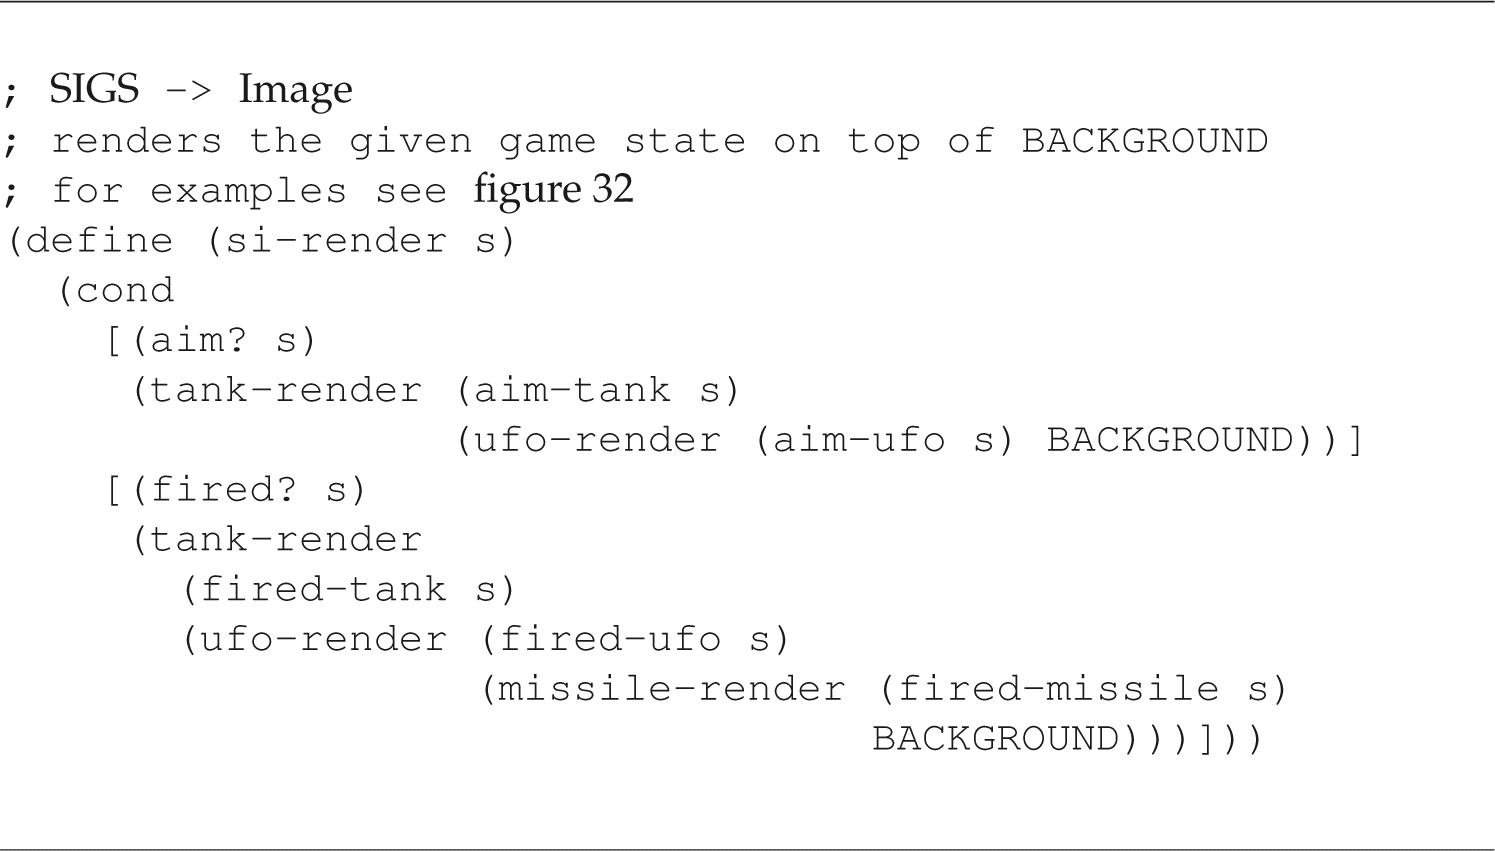
\includegraphics[width=0.85\textwidth]{images/00122.png}
  \caption{包含结构体的完整渲染函数 si-render（注：代码注释中原书连续编号 Figure 32 对应本书图 6.2）}
  \label{fig:sigs_render_full}
\end{figure}

观察图~\ref{fig:sigs_render_full} 中的 \code{si-render} 函数。由于输入参数 \code{s} 是一个分类数据，函数顶层由一个 \code{cond} 表达式统领，分别利用谓词 \code{aim?} 与 \code{fired?} 区分具体属于哪种结构体；在每个分支内部，则严格遵循结构体设计配方，提取各字段选择器进行下层图像合成。

\begin{exercise}{游戏场景与常数设计}{94}
绘制太空侵略者游戏在不同阶段的若干场景草图。据此确定游戏中的不变常数与可变量：定义画布尺寸常数（\code{WIDTH}, \code{HEIGHT}）、UFO 图像、坦克图像、导弹图像以及背景画布 \code{BACKGROUND}。
\end{exercise}

\begin{exercise}{分析游戏状态实例}{95}
解释为什么以下三个实例分别属于数据定义的第一个或第二个分支：
\begin{lstlisting}[language=BSL]
(make-aim (make-posn 20 10) (make-tank 28 -3))
(make-fired (make-posn 20 10) (make-tank 28 -3) (make-posn 28 (- HEIGHT TANK-HEIGHT)))
(make-fired (make-posn 20 100) (make-tank 100 3) (make-posn 22 103))
\end{lstlisting}
\end{exercise}

\begin{exercise}{绘制游戏场景草图}{96}
在 $200 \times 200$ 的画布坐标系中，手动绘制练习~\ref{ex:95} 中三个状态分别对应的游戏渲染画面。
\end{exercise}

\begin{exercise}{设计分层渲染辅助函数}{97}
遵循辅助函数设计原则，分别设计 \code{tank-render}、\code{ufo-render} 与 \code{missile-render}，并用它们装配出高内聚、低耦合的 \code{si-render}。
\end{exercise}

\begin{exercise}{胜负终止判断 si-game-over?}{98}
设计游戏结束判断函数 \code{si-game-over?}。游戏在发生以下任一情况时终止：
\begin{enumerate}
  \item UFO 触地着陆（即其纵坐标达到或超过 \code{HEIGHT}）；
  \item 导弹成功命中 UFO（即导弹坐标与 UFO 坐标距离足够接近，例如小于 5 像素）。
\end{enumerate}
此外，设计游戏终盘画面渲染函数 \code{si-render-final}，在屏幕上醒目展示游戏结果。
\end{exercise}

\begin{exercise}{移动更新函数 si-move}{99}
设计时钟滴答处理函数 \code{si-move}：
\begin{itemize}
  \item 坦克沿水平方向以当前速度匀速移动；
  \item 导弹（若已发射）垂直向上高速直线运动；
  \item UFO 垂直匀速下落，并在水平方向进行小幅随机跳跃（借助 BSL 内置的 \code{random} 函数）。
\end{itemize}
\end{exercise}

\begin{exercise}{按键控制函数 si-control}{100}
设计按键事件处理函数 \code{si-control}，响应以下三颗按键：
\begin{itemize}
  \item \code{"left"}：改变坦克速度方向向左；
  \item \code{"right"}：改变坦克速度方向向右；
  \item 空格键 \code{"\ "}：若导弹尚未发射，则在坦克顶部点火生成一枚新导弹！若导弹已在飞行中，则忽略此按键。
\end{itemize}
\end{exercise}

\begin{exercise}{自动化测试全覆盖}{101}
将图~\ref{fig:space_invader_render_examples} 与图~\ref{fig:sigs_render_full} 中的示例转化为严格的 \code{check-expect} 单元测试。
\end{exercise}

\subsection{另一种数据表示方案：单一结构体与可选字段}

作为对比，我们也可以将游戏状态建模为一个包含三字段的统一结构体：

\begin{lstlisting}[language=BSL]
(define-struct sigs [ufo tank missile])
; 一个 SIGS.v2 是一个结构体：
;   (make-sigs Posn Tank MissileOrNot)
; 一个 MissileOrNot 是以下两者之一：
; -- #false
; -- Posn
; 解释：#false 表示尚未发射导弹；Posn 表示导弹当前坐标
\end{lstlisting}

\begin{figure}[htbp]
  \centering
  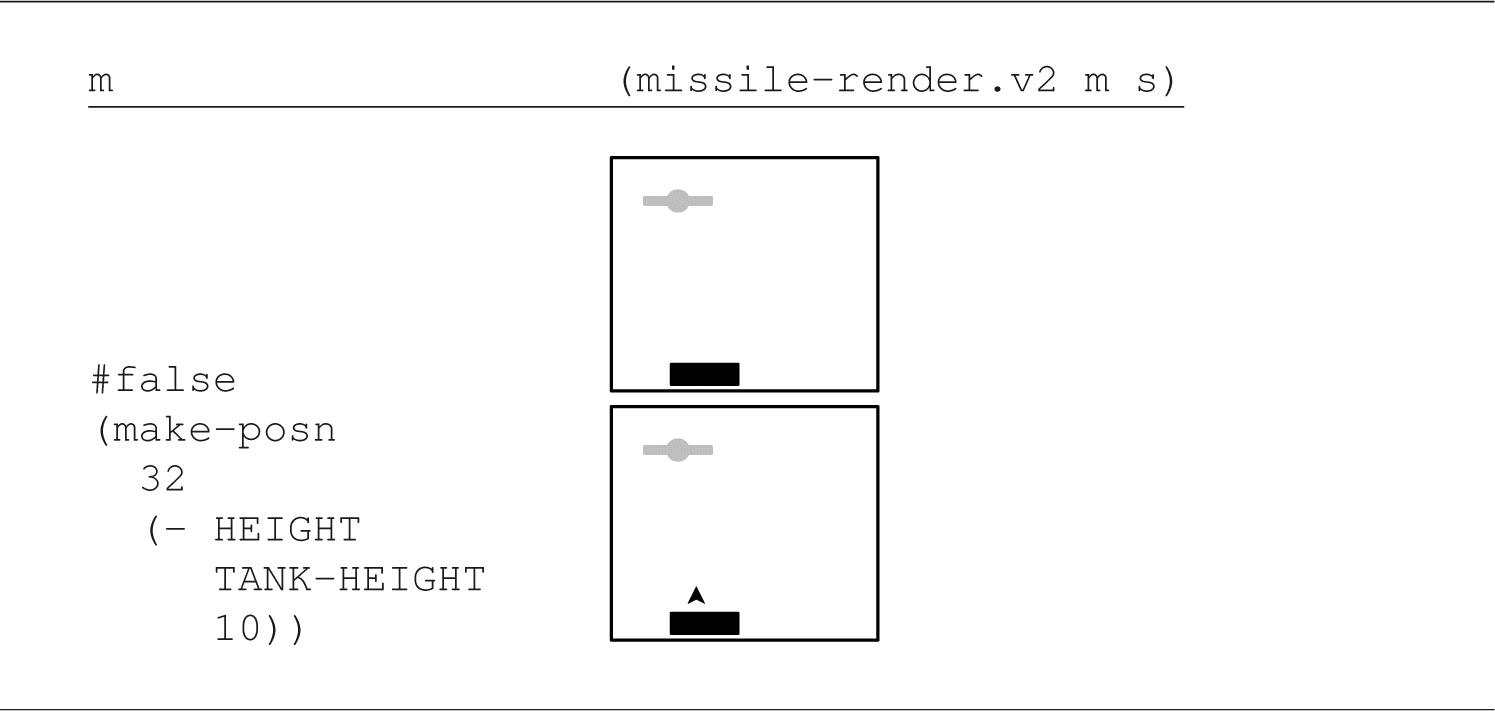
\includegraphics[width=0.85\textwidth]{images/00126.png}
  \caption{第二种游戏状态数据表示下的渲染函数}
  \label{fig:sigs_v2_render}
\end{figure}

\begin{exercise}{完成第二种方案的代码}{102}
基于 \code{SIGS.v2} 数据表示，重新设计太空侵略者游戏的所有核心事件处理函数。
\end{exercise}

\begin{exercise}{动物园管理系统}{103}
设计一套结构体与分类数据，用于表示动物园中的四种动物：蜘蛛（记录剩余腿数与运输体积）、大象（记录空间需求）、蟒蛇（记录长度与腰围）和犰狳（记录体重与铠甲硬度）。设计函数 \code{fits?} 判断某只动物是否能装入给定制式的笼子。
\end{exercise}

\begin{exercise}{车辆分类系统}{104}
为包含小汽车、货车、大巴和 SUV 的车队设计结构体与分类数据定义，并编写函数计算过路费。
\end{exercise}

\begin{exercise}{广义坐标 Coordinate}{105}
考虑如下数据定义：
\begin{lstlisting}[language=BSL]
; 一个 Coordinate 是以下两者之一：
; -- 一个非负数 Number
; -- 一个 Posn
; 解释：单个数字表示位于数轴上的点；Posn 表示平面二维点
\end{lstlisting}
设计函数 \code{distance-to-origin}，计算任意 \code{Coordinate} 到坐标原点的欧几里得距离。
\end{exercise}

% ==============================================================================
\section{混合型世界程序}
\label{sec:6.2_mixing_up_worlds}
% ==============================================================================

在第 5.11 节中，我们分别设计了小猫与变色龙。如果我们希望在一个程序中让用户自主选择领养哪种宠物，世界状态本身就必须是一个分类数据！

\begin{figure}[htbp]
  \centering
  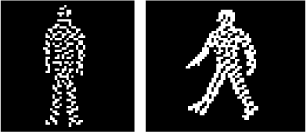
\includegraphics[width=0.75\textwidth]{images/00127.png}
  \caption{混合虚拟宠物游戏原型}
  \label{fig:mixed_pet_prototype}
\end{figure}

\begin{exercise}{统一宠物世界 VAnimal}{106}
定义分类数据 \code{VAnimal}：
\begin{lstlisting}[language=BSL]
; 一个 VAnimal 是以下两者之一：
; -- VCat
; -- VCham
\end{lstlisting}
设计世界程序，在画布上渲染当前激活的宠物，并处理其饥饿流逝与按键抚摸互动。
\end{exercise}

\begin{exercise}{猫与变色龙双宠乐园}{107}
设计一个同时容纳小猫和变色龙的双宠世界程序 \code{cham-and-cat}。定义一个包含两个宠物的结构体，让它们在同一张画布上并排漫步。
\end{exercise}

\begin{exercise}{行人过街信号灯倒计时}{108}
设计一个逼真的行人过街交通灯：
\begin{itemize}
  \item 默认状态：红色背景，站立的橙色小人；
  \item 收到通行信号：切换为绿色背景，行走的绿色小人，持续 10 秒；
  \item 随后进入数字倒计时：显示数字 $9, 8, \dots, 0$。奇数显示为橙色，偶数显示为绿色；
  \item 倒计时归零后切回默认禁行状态。
\end{itemize}
\end{exercise}

\begin{exercise}{按键序列模式识别机}{109}
设计一个识别特定按键序列的世界程序：初始显示 $100 \times 100$ 的白色方块；当用户按下首个目标字符时变为黄色；输入完最终字符后变为绿色；若在任何步骤输入错误按键，则方块立即变红报警。
\end{exercise}

% ==============================================================================
\section{输入错误与防御性设计}
\label{sec:6.3_input_errors}
% ==============================================================================

在此前的所有函数设计中，我们默认函数的调用者都是“守规矩”的合作者——传递的实参类型完全符合函数签名。但在真实生产环境中，函数随时可能遭遇非法实参的恶意或误操作调用。

如果一个计算圆面积的函数被传递了字符串 \code{"five"} 或负数 $-10$：
\begin{lstlisting}[language=BSL]
(define (area-of-disk r)
  (* 3.14 (sqr r)))
\end{lstlisting}
传递 \code{"five"} 会引发底层原始算术操作符的崩溃，而传递 $-10$ 甚至会静默地输出一个看似合理但物理错误的答案！

BSL 提供了 \code{error} 函数用于显式抛出运行时错误，并提供了 \code{check-error} 用于对错误处理进行单元测试：

\begin{lstlisting}[language=BSL]
; Any -> Number
; 带防御性参数校验的圆盘面积计算函数
(check-expect (checked-area-of-disk 2) (* 3.14 4))
(check-error (checked-area-of-disk "two") "area-of-disk: number expected")
(check-error (checked-area-of-disk -3) "area-of-disk: positive number expected")

(define (checked-area-of-disk v)
  (cond
    [(and (number? v) (>= v 0)) (area-of-disk v)]
    [(not (number? v)) (error "area-of-disk" "number expected")]
    [else (error "area-of-disk" "positive number expected")]))
\end{lstlisting}

\begin{exercise}{校验正数面积输入}{110}
完整实现并测试 \code{checked-area-of-disk}，确保其在输入合法正数、零、负数以及非数值类型时均给出精确的行为。
\end{exercise}

\begin{exercise}{防御性二维向量构造}{111}
考虑结构体 \code{(define-struct vec [x y])}。设计函数 \code{checked-make-vec}，校验两个坐标分量必须均为正数，否则抛出详尽的错误提示。
\end{exercise}

% ==============================================================================
\section{检查世界状态}
\label{sec:6.4_checking_the_world}
% ==============================================================================

在调试复杂的世界程序时，程序崩溃常常发生在某个深层子函数中，但真正的罪魁祸首却是上一轮时钟滴答生成的非法世界状态。

为了捍卫系统边界，我们应当为每一个自定义数据定义编写\term{类型识别谓词}（Type Predicates）：

\begin{lstlisting}[language=BSL]
; Any -> Boolean
; 判定给定值是否为一个合法的导弹发射阶段状态
(define (fired-state? v)
  (and (fired? v)
       (posn? (fired-ufo v))
       (tank? (fired-tank v))
       (posn? (fired-missile v))))
\end{lstlisting}

\begin{exercise}{使用 or 重构谓词}{112}
使用 \code{or} 表达式重构复合类型判定函数，使其逻辑更加精炼。
\end{exercise}

\begin{exercise}{为核心数据定义编写谓词}{113}
分别为前文中的 \code{SIGS}、\code{Coordinate} 以及 \code{VAnimal} 设计完整的类型验证谓词。
\end{exercise}

\begin{exercise}{全面装备世界程序}{114}
使用练习~\ref{ex:113} 中编写的谓词，为太空侵略者、虚拟宠物以及文本编辑器世界程序装配状态自检断言。
\end{exercise}

% ==============================================================================
\section{相等性谓词}
\label{sec:6.5_equality_predicates}
% ==============================================================================

BSL 为基本类型提供了各自的相等性比较函数：\code{=} 用于比较数，\code{string=?} 用于比较字符串，\code{boolean=?} 用于比较布尔值。但对于程序员自定义的枚举与结构体，BSL 并没有提供开箱即用的比对函数。

考虑第 4.7 节中的交通信号灯枚举 \code{TrafficLight}。要判断两个交通信号灯状态是否完全一致，我们应当遵循设计配方编写专属的相等性谓词：

\begin{lstlisting}[language=BSL]
; TrafficLight TrafficLight -> Boolean
; 判断两盏交通信号灯的状态是否相同
(check-expect (light=? "red" "red") #true)
(check-expect (light=? "red" "green") #false)
(check-expect (light=? "green" "green") #true)
(check-expect (light=? "yellow" "yellow") #true)

(define (light=? a-light another-light)
  (string=? a-light another-light))
\end{lstlisting}

如果我们希望进一步增强该函数的鲁棒性，让它在接收到非信号灯字符串时主动报错，便可以借助前文的错误校验机制：

\begin{exercise}{智能报错的信号灯比较谓词}{115}
修改 \code{light=?} 函数，使其在遇到非法输入时不仅抛出错误，还能在错误消息中明确指出究竟是第几个实参不是合法的 \code{TrafficLight}。
\end{exercise}
